\documentclass{beamer}
%\usetheme{Boadilla}

\usepackage[utf8]{inputenc}
\usepackage[french]{babel} %pour la typographie française.
\usepackage[T1]{fontenc} %pour la césure des mots.
\usepackage{amssymb} %pour les symboles mathématiques et lettres grecques
\usepackage{amsmath} %pour les formules mathématiques avancées
\usepackage{listings} %lstlisting
\usepackage{xcolor} % pour mettre du texte en couleur
\usepackage{tikz}
\usetikzlibrary{calc, trees, positioning, arrows, shapes, shapes.multipart, shadows, matrix, decorations.pathreplacing, decorations.pathmorphing, automata, decorations.markings}
\definecolor{vert}{RGB}{0,153,0}

\beamertemplatenavigationsymbolsempty % Option pour supprimer la barre de navigation dans les slides

\title{Projet TriComp : Présentation}
\author{Equipe TriComp}
\date{Jeudi 18 Décembre 2014}

% Faire apparaître un sommaire avant chaque section
\AtBeginSection[]{
   \begin{frame}{Plan}
%   \begin{center}{\Large Plan }\end{center}
   %%% affiche en début de chaque section, les noms de sections et
   %%% noms de sous-sections de la section en cours.
   \tableofcontents[currentsection]
   \end{frame}
}

\setbeamertemplate{footline}[frame number]

\tikzstyle{vecArrow} = [thick, decoration={markings,mark=at position
   1 with {\arrow[semithick]{open triangle 60}}},
   double distance=1.4pt, shorten >= 5.5pt,
   preaction = {decorate},
   postaction = {draw,line width=1.4pt, white,shorten >= 4.5pt}]
\tikzstyle{innerWhite} = [semithick, white,line width=1.4pt, shorten >= 4.5pt]

\begin{document}

\frame{
   \begin{center}
        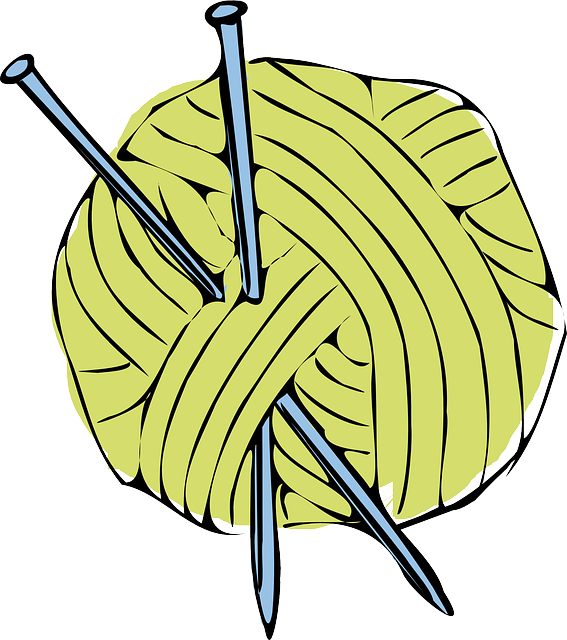
\includegraphics[height=0.2\textheight]{../img/ball_of_wool.png}
        \hspace*{4cm}
        
\includegraphics[height=0.2\textheight]{../img/logo_ens.jpg}
   \end{center}
   \titlepage
}

\frame{
	\frametitle{Plan}
		\tableofcontents
}

\section{Introduction}

\frame{
	\frametitle{L'équipe TriComp}
		\begin{center}
			{\large
			{William \textsc{Aufort} \hspace{4cm} Julien \textsc{Bensmail} \\}
			\vspace{1cm}
			{Agathe \textsc{Herrou}  \hspace{4cm} Romain \textsc{Labolle} \\}
			\vspace{1cm}
			{Frédéric \textsc{Lang} \hspace{4cm} Maxime \textsc{Lesourd} \\}
			\vspace{1cm}
			{Laureline \textsc{Pinault} \hspace{3.7cm} Léo \textsc{Stéfanesco} \\}}
		\end{center}
}

\subsection{Motivations}

\frame{

  \frametitle{Motivations}
  \begin{itemize}
    \onslide<2-> \item Tricot peu présent dans le milieu informatique
    \onslide<3-> \item Logiciels de tricot incomplets : pas d'instructions
    \onslide<4-> \item Représentation inefficace des tricots (matrices de points)
    % Deux raisons d'automatiser le calcul des instructions
    \onslide<5-> \item Instructions longues, fastidieuses à établir
    \onslide<6-> \item Ne tiennent pas compte de la forme du tricot dans les ouvrages.
    \onslide<7-> \item Un projet original !
  \end{itemize}
}

\subsection{Quelques notions de tricot}

\frame{
	\frametitle{Quelques notions de tricot...}
	\begin{center}
	  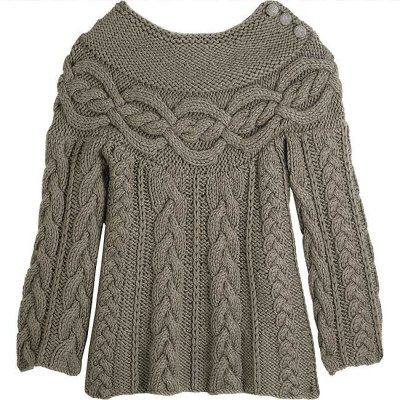
\includegraphics[scale=0.75]{pulltorsadesecossaises.jpg}
	\end{center}
}

\frame{
  \frametitle{Zoomons}
  
  \begin{columns}

    \begin{column}{0.5\textwidth}

  \begin{center}
    \begin{figure}
    \includegraphics[scale=0.04]{../img/Stockinette_example_front.JPG}
    \caption{Jersey endroit}
    \end{figure}
  \end{center}
  
    \end{column}
    
    \begin{column}{0.5\textwidth}

  \begin{center}
    \begin{figure}
    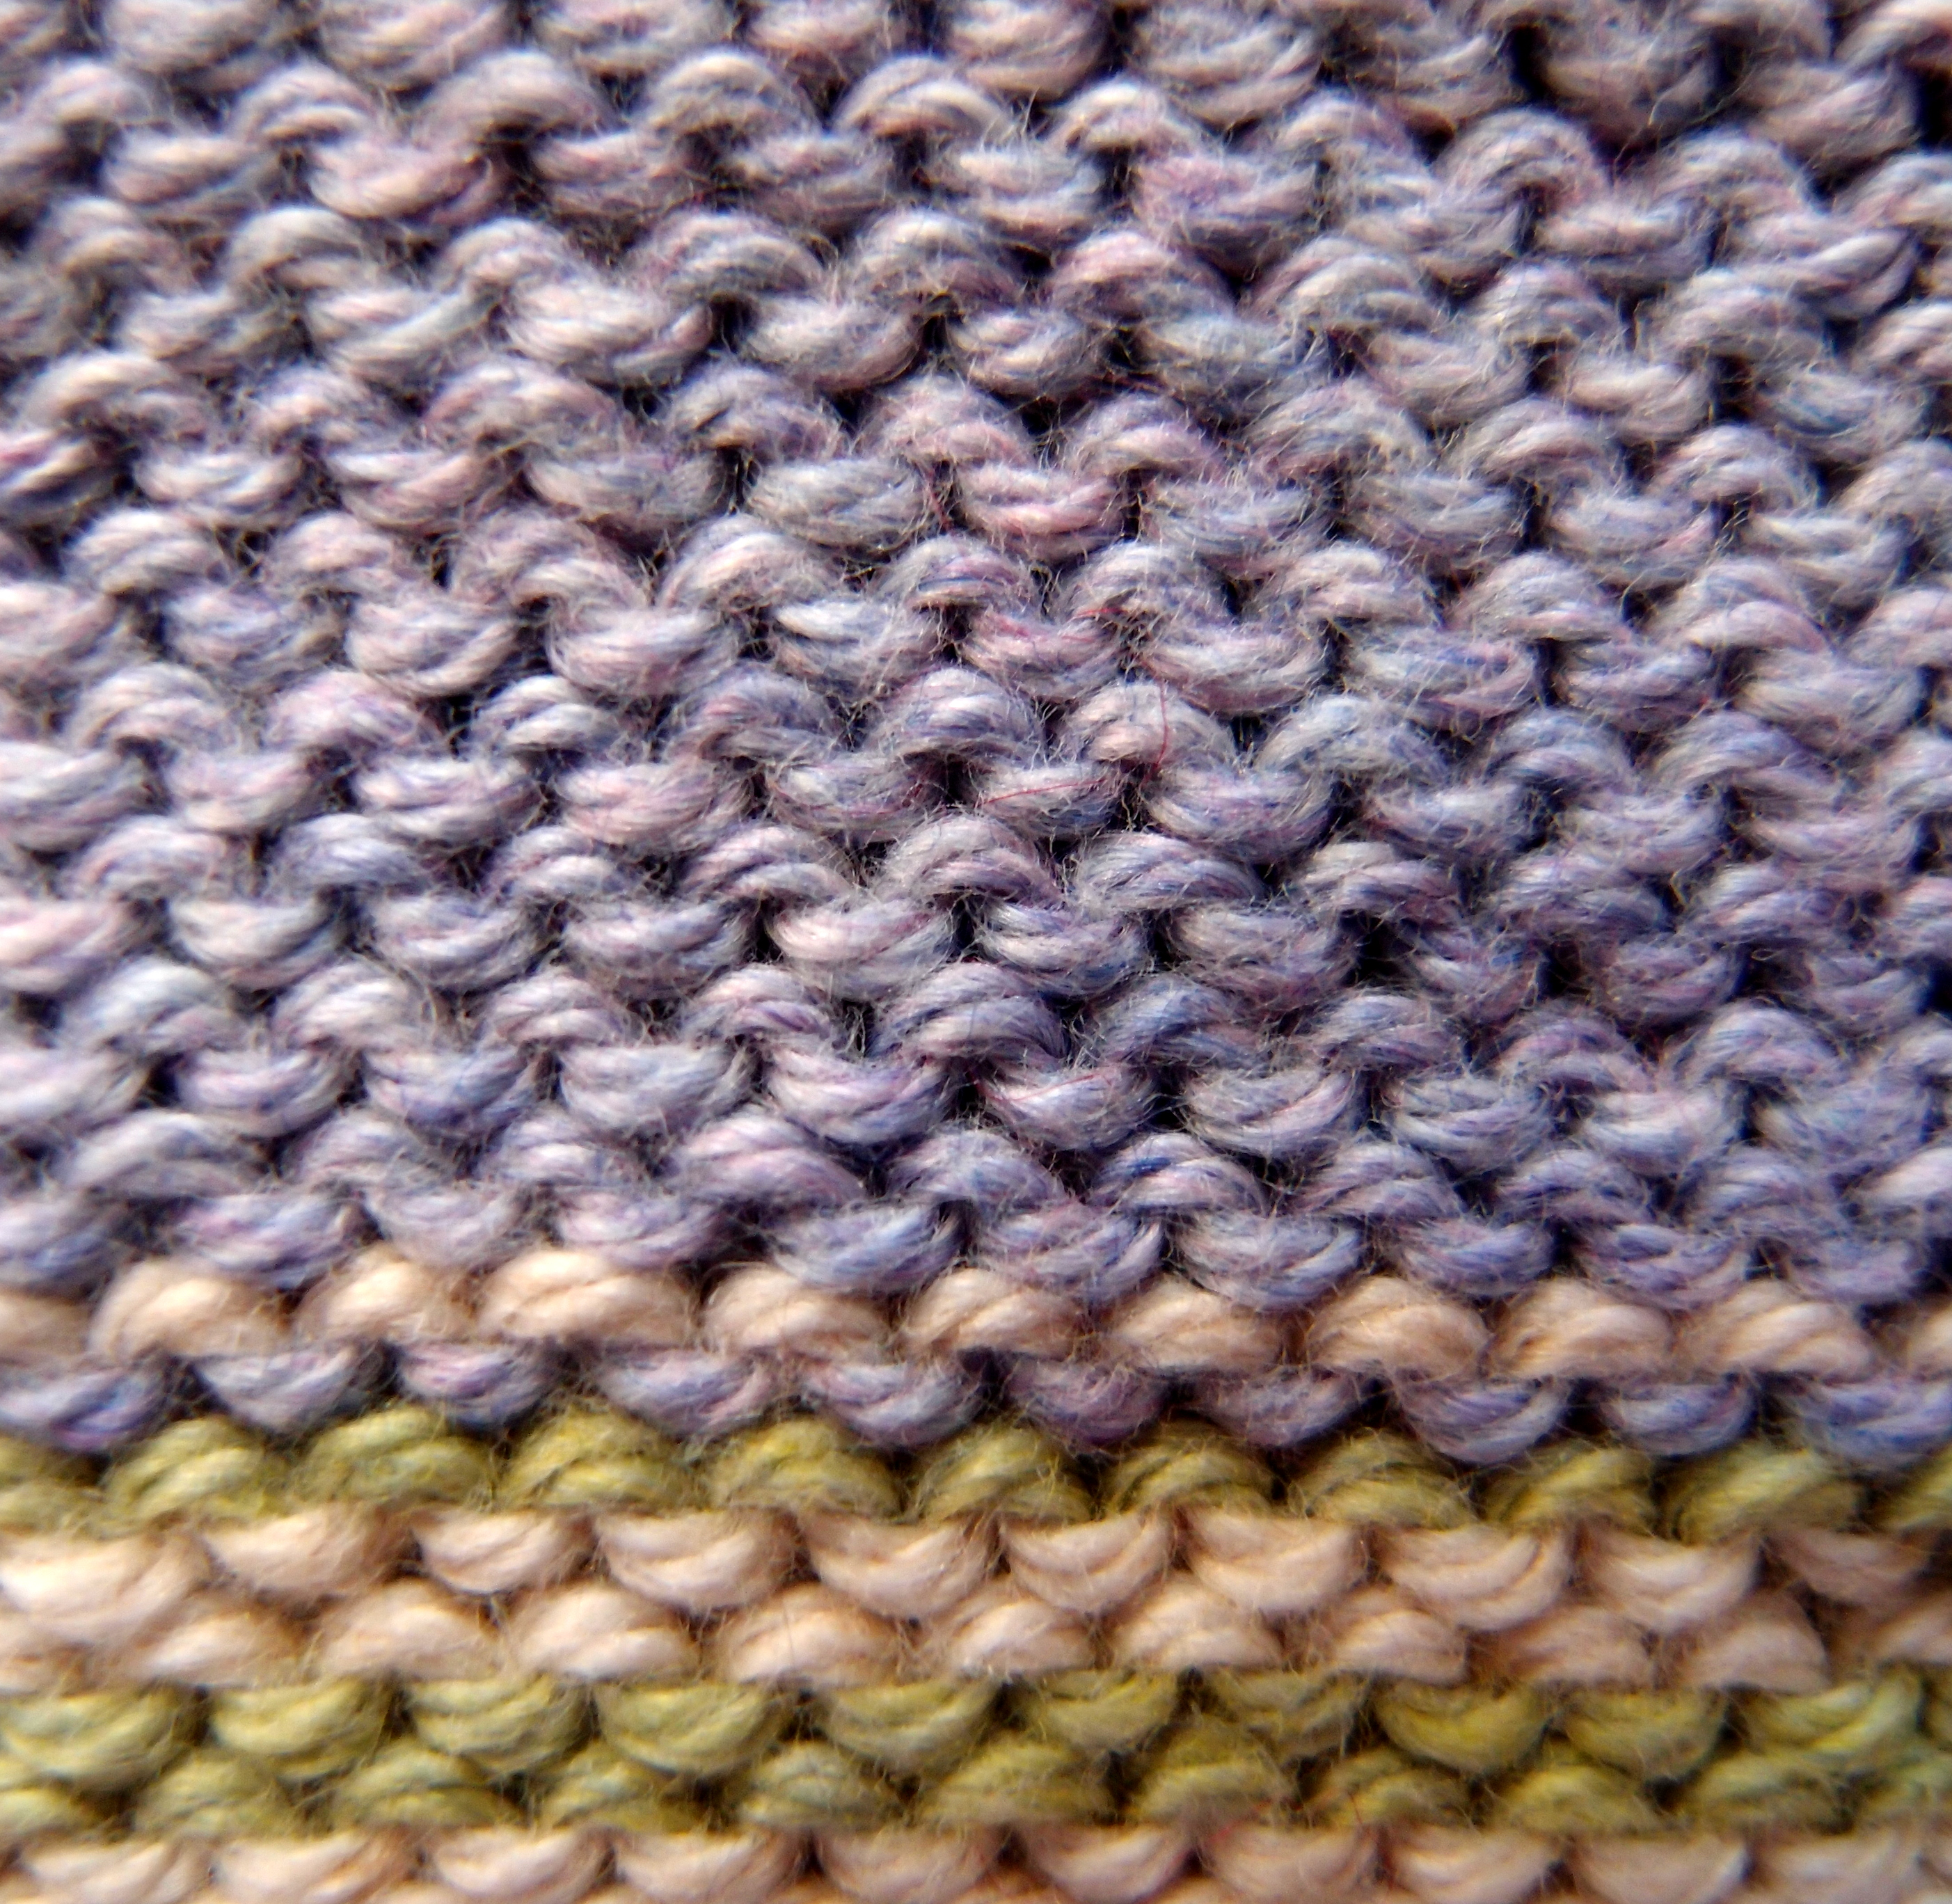
\includegraphics[scale=0.04]{../img/Stockinette_example_back.JPG}
    \caption{Jersey envers}
    \end{figure}    
  \end{center}
  
    \end{column}
  \end{columns}
}

\frame{
	\frametitle{Zoomons}
        \begin{columns}   
          \column{0.6\textwidth}
          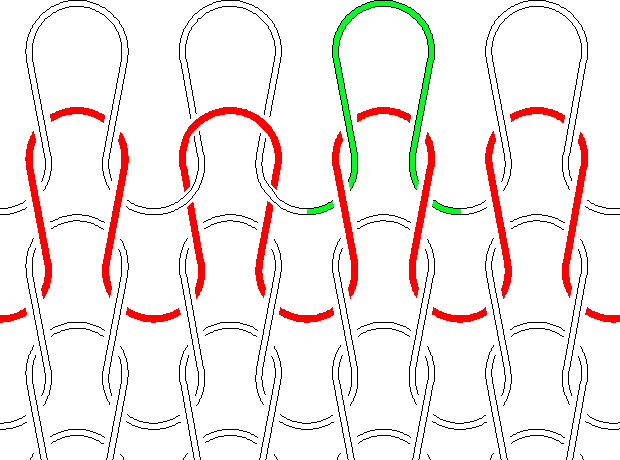
\includegraphics[scale=0.3]{Knit-schematic.png}
          \column{0.4\textwidth}
          \begin{itemize}
            \pause
          \item[] \textcolor{green}{maille}
            \pause
          \item[] \textcolor{red}{rang}
          \end{itemize}
        \end{columns}
}

\frame{
	\frametitle{Zoomons}
        \begin{columns}   
          \column{0.6\textwidth}
          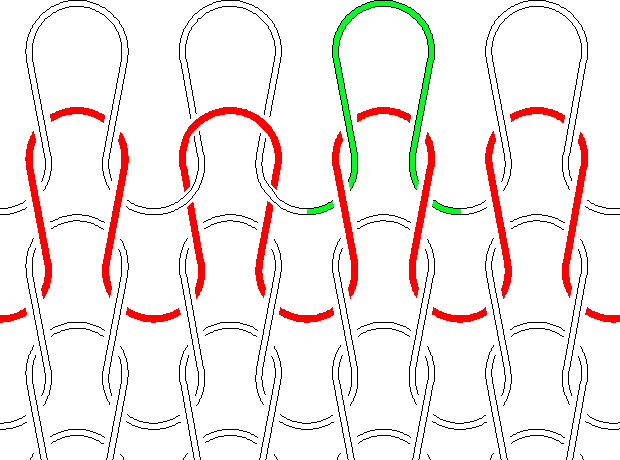
\includegraphics[scale=0.3]{Knit-schematic.png}
          \column{0.4\textwidth}
          \begin{itemize}
          \item[] \textcolor{green}{maille à l'endroit}
          \item[]
          \end{itemize}
        \end{columns}
}
\frame{
	\frametitle{Zoomons}
        \begin{columns}   
          \column{0.6\textwidth}
          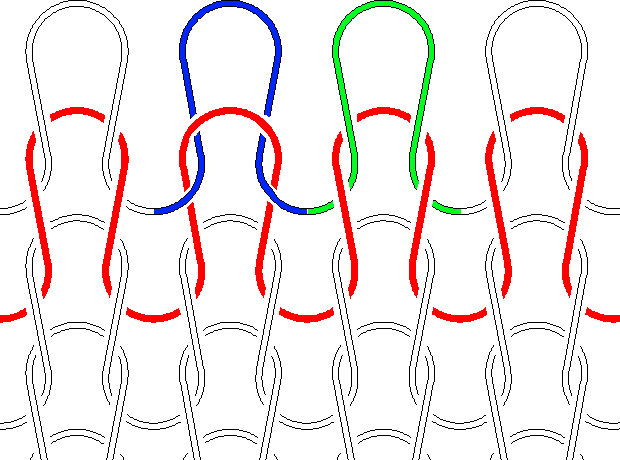
\includegraphics[scale=0.3]{Knit-schematic2.png}
          \column{0.4\textwidth}
          \begin{itemize}
          \item[] \textcolor{green}{maille à l'endroit}
          \item[] \textcolor{blue}{maille à l'envers}
          \end{itemize}
        \end{columns}
}



\frame{
	\frametitle{Les instructions de tricot}
			Les instructions à suivre par le tricoteur comportent des informations sur :
			\begin{itemize}
				\item le type de point à tricoter
				\item le nombre de points identiques
				\item le nombre de rangs à reproduire
			\end{itemize}
                        $\Rightarrow$ Description d'un motif minimal à répéter
			% TODO : Un exemple d'instructions de tricot
}

\subsection{Présentation générale}

\frame{
	\frametitle{TriComp : un compilateur pour tricot}
	\begin{figure}[!h]
		\centering
		\begin{tikzpicture}[->, >=stealth', shorten >=1pt, auto, node distance = 3.5cm, semithick]
			\tikzstyle{every state}=[draw=black,text=black,shape=rectangle]
		    \node[single arrow, draw, align=center, xshift=0cm, yshift=5cm, rotate=0, minimum height=4em](compilateur)[xshift=-1cm]
				{Compilateur};
%		    \node[state] (compilateur) [shape=arrow] 	{Compilateur};
		    \node[rectangle, draw, minimum height=10em, minimum width=7em, align=center](patron-d)[left of=compilateur,xshift=0.5cm]
				{\textit{Liste des pièces}\\ \textit{Forme} \\ \textit{Motif} \\ \textit{Taille}};
%		    \node[state] (patron-d) [] [left of=compilateur] {\textit{Liste des pièces}};
		    \node[rectangle, draw, minimum height=10em, minimum width=7em, align=center](instructions-d)[right of=compilateur]
				{\noindent \texttt{1 maille endroit} \\ \texttt{3 mailles envers} \\ \texttt{...}};
%		    \node[state] (instructions-d) [] [right of=compilateur] {\textit{Liste des instructions}};
		    \node[state] (patron) [draw=none] 	[above of=patron-d, yshift=-2cm] {Patron du tricot};
		    \node[state] (instructions) [draw=none] [above of=instructions-d,  yshift=-2cm]	{Instructions};
		\end{tikzpicture}
	\end{figure}
	\hspace{3cm}
	\pause
	\begin{center}
		Le tout utilisable via une interface graphique
	\end{center}
}

\frame{
    \frametitle{Fonctionnement du logiciel}
        \begin{figure}[!h]
    \centering
\begin{tikzpicture}[thick,node distance= 2.5cm]
  \node[draw=none] (u) {Utilisateur};
  \node[draw,rectangle, below of=u] (a) {Description du tricot};
  \node[inner sep=0,minimum size=0,right of=a] (k) {}; % invisible node
  \node[draw,rectangle,right of=k] (b) {Rendu visuel du patron};
  \node[draw,rectangle,below of=a] (c) {Instructions pour tricoter};
  \node [draw=none, below right of=k, node distance=1.75cm] {Compilateur};

  % 1st pass: draw arrows
  \draw[vecArrow] (u) -- node [right] {TriLang} ++ (a) ;
  \draw[vecArrow] (a) -- node [above] {GUI} ++ (b) ;
  \draw[vecArrow] (k) |-  (c) ;

  % 2nd pass: copy all from 1st pass, and replace vecArrow with innerWhite
  \draw[innerWhite] (a) to (b);
  \draw[innerWhite] (k) |- (c);

  % Note: If you have no branches, the 2nd pass is not needed
\end{tikzpicture}
    \end{figure}    
    }


\section{Notre travail}

\subsection{Conception d'un langage descriptif}

\frame{
	\frametitle{En amont... description d'un tricot}
	
		Objectifs :
		\begin{itemize}
			\item Pouvoir décrire n'importe quel tricot
			\item Description globale	    % i.e : suffisamment précis pour avoir du détail, mais conserver un aspect global,
							    % contrairement à ce qui se fait d'habitude dans les logiciels de tricots
			        			    % (points sur une grille)
			\item Facilité pour générer les instructions
			\item Facilité de prise en main
		\end{itemize}
%			Nous avons donc conçu le langage \textsc{TriLang} % TODO : meilleur nom ?
}

\frame{
	\frametitle{Le langage}
		\begin{itemize}
			\item La composante essentielle : le trapèze \\
			\begin{center}
				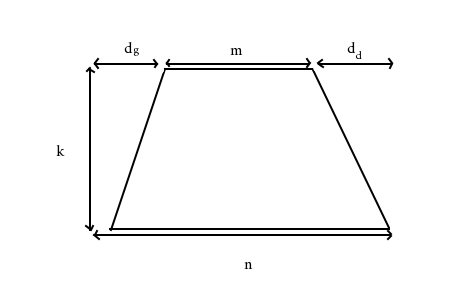
\includegraphics[height=0.4\textheight]{../img/trapeze.jpg}
			\end{center}
			\item Chaque trapèze pointe vers l'entité suivante $\rightarrow$ parcours facile du tricot
			\item Pour relier/séparer des pièces : \texttt{link} et \texttt{split}
		\end{itemize}
}

\frame{
	\frametitle{Un exemple}

	\begin{center}
	\begin{tikzpicture}[scale = 0.05]
		\tikzstyle{fleche}=[->,>=latex,line width=1mm]
		\fill[color=gray!20] (0,0) -- (60,0) -- (60,120) -- (0,120) -- cycle;
		\fill[color=white] (30,30) -- (45,60) -- (30,90) -- (15,60) -- cycle;
		\draw[thick] (0,0) -- (60,0) -- (60,120) -- (0,120) -- cycle;
		\draw[thick] (0,30) -- (60,30) ;
		\draw[thick] (0,90) -- (60,90) ;
		\draw[thick] (0,60) -- (15,60) ;
		\draw[thick] (45,60) -- (60,60) ;
		\draw[thick] (30,30) -- (45,60) -- (30,90) -- (15,60) -- cycle;

		\onslide<2->
		\draw[fleche, color=red] (30,20) -- (15,40);
		\draw[fleche, color=red] (30,20) -- (45,40);
		\draw[color=red] (30,15) node{split};
		\draw[fleche, color=blue] (8,50) -- (8,70);
		\draw[fleche, color=blue] (52,50) -- (52,70);
		\draw[color=blue] (30,60) node{next};
		\draw[fleche,color=green] (15,80) -- (30,100);
		\draw[fleche,color=green] (45,80) -- (30,100);
		\draw[color=green] (30,105) node {link};
		\draw (30,-10) node{start};
		\draw[fleche] (30,-5) -- (30,10);
		\draw (30,130) node{stop};
		\draw[fleche] (30,110) -- (30,125);
		\draw[-*,ultra thick] (75,30) -- (45,15);
		\draw (90,35) node{\texttt{trapeze(...)}};
	\end{tikzpicture}
	\end{center}
}

\subsection{Conception d'un compilateur}

\frame{
	\frametitle{Le compilateur}
		\begin{itemize}
			\onslide<1-> \item Génère la liste d'instructions.
			\onslide<2-> \item Détection d'erreurs (cycles, configurations impossibles).
			\onslide<3-> \item Principale difficulté : Certaines pièces dépendent d'autres.
			\onslide<4-> \item Parcours selon un ordre topologique.
		\end{itemize}
}

\frame{
	\frametitle{Exemple}

	\begin{center}
	\begin{tikzpicture}[scale = 0.05]
		\tikzstyle{fleche}=[->,>=latex,line width=1mm]
		\fill[color=gray!20] (0,0) -- (60,0) -- (60,120) -- (0,120) -- cycle;
		\fill[color=white] (30,30) -- (45,60) -- (30,90) -- (15,60) -- cycle;
		\draw[thick] (0,0) -- (60,0) -- (60,120) -- (0,120) -- cycle;
		\draw[thick] (0,30) -- (60,30) ;
		\draw[thick] (0,90) -- (60,90) ;
		\draw[thick] (0,60) -- (15,60) ;
		\draw[thick] (45,60) -- (60,60) ;
		\draw[thick] (30,30) -- (45,60) -- (30,90) -- (15,60) -- cycle;

%		\draw[fleche, color=red] (30,20) -- (15,40);
%		\draw[fleche, color=red] (30,20) -- (45,40);
%		\draw[color=red] (30,15) node{split};
%		\draw[fleche, color=blue] (8,50) -- (8,70);
%		\draw[fleche, color=blue] (52,50) -- (52,70);
%		\draw[color=blue] (30,60) node{next};
		\draw[fleche,color=green] (15,80) -- (30,100);
		\draw[fleche,color=green] (45,80) -- (30,100);
		\draw[color=green] (30,105) node {link};
%		\draw (30,-10) node{start};
%		\draw[fleche] (30,-5) -- (30,10);
%		\draw (30,130) node{stop};
%		\draw[fleche] (30,110) -- (30,125);
	\end{tikzpicture}
	\end{center}
	
}

\frame{
  \frametitle{Implémentation actuelle}
        \begin{itemize}
          \onslide<1-> \item Compilation et vérification.
          \onslide<2-> \item Limité à des rectangles.
          \onslide<3-> \item \textcolor{vert}{Algorithmes pour les réductions/augmentations de motifs.}
          \onslide<4-> \item Motifs prédéfinis.
          \onslide<5-> \item \textcolor{vert}{Format extensible.}
          \onslide<6-> \item Utilisable en ligne de commande ou à travers l'interface.
        \end{itemize}

}

\subsection{Elaboration d'une interface}

\frame{
	\frametitle{L'interface graphique}
		3 objectifs :
		\begin{itemize}
			\item Simple d'utilisation
			\item Outils d'éditions
			\item Appel au compilateur
		\end{itemize}
}

\frame{
	\begin{center}
		\Huge{Démo !}
	\end{center}
}

\section{Difficultés rencontrées \& améliorations possibles}

\subsection{Difficultés}

\frame{
	\frametitle{Difficultés rencontrées}
		\begin{itemize}
			  	\onslide<2-> \item \textcolor{red}{Première étape de conception du langage sous-estimée...} \\
				\onslide<3-> \textcolor{vert}{$\longrightarrow$ mais un langage plus complet dès le début}
				\onslide<4-> \item \textcolor{red}{Conception de l'interface $\rightarrow$ temps nécessaire}
				\onslide<5-> \item \textcolor{red}{Mise en route difficile...} \\
				\onslide<6-> \textcolor{vert}{$\longrightarrow$ mais beaucoup de simplifications effectuées depuis la proposition}
    	\end{itemize}
}

\subsection{Améliorations}

\frame{
  \frametitle{Améliorations en perspective...}
  \begin{itemize}
    \onslide<2-> \item Édition : plus de liberté dans la personnalisation
    \begin{itemize}
      \item Des points définis par l'utilisateur
      \item Pouvoir ajouter des tresses \\
		$\longrightarrow$ Définition de zones sur les trapèzes ?
	\item Gérer les coutures (à effectuer après le tricot)
    \end{itemize}
    \onslide<3-> \item Compilateur :
    \begin{itemize}
      \item Implémenter la répartition des augmentations et des diminutions
    \end{itemize}
  \onslide<4-> \item Interface graphique : 
    \begin{itemize}
     \item Plus de modifications du tricot possibles (changer la taille des pièces,...)
     \item Pouvoir créer son tricot dans l'interface
    \end{itemize}

  \end{itemize}
}

\frame{
	\begin{center}
		\Huge{Des questions ?}
	\end{center}
}

\end{document}
